% Provenance (never printed): see sources/outline_sources.md (Year 2: sedimentary basins;
% subsidence curves and backstripping; the stretching model). Stretching model after McKenzie
% (1978) as restated by Sheplev and Reverdatto (1998) and coded in pyBacktrack (EarthByte);
% backstripping after pyBacktrack's well module; North Sea after Sclater and Christie (1980);
% Michigan after Sloss (1982) and Crowe et al. (2009); the US Atlantic margin after Schlee et
% al. (1976), Poag (1979) and Lang et al. (2024); the Molasse after the chapter 13 rows.
% Curves and the invented well from figdata/bachelor-2/basins.py; exercise and problem values
% in the Book 4 scratch calculator calc/ch16.py.
 \chapter{沉积盆地比较}\label{ch:b2:basins-compared}

美国东部海岸外，大陆架之下，巴尔的摩
峡谷海槽中至少有 \qty{14}{km} 厚的沉积岩。钻孔打入这样的
沉积层序时，其历史是倒着读的：所穿过的每一层，曾经都是海底，
当时的深度由化石和沉积物记录，此后被掩埋、挤压。每一个定年界面的
深度，都是\omterm{def:b2:basins-compared:curve}{沉降曲线}上的一个点。然而，大部分沉降是由
沉积物自身的重量造成的。要弄清盆地是怎样形成的，就必须把这部分重量
逐层扣除。本章说明具体做法，以及结果对岩石圈说明了什么。
% ledger: poag79:bct, schlee76:atlantic

\begin{recall}
\textbf{来自本科一年级分册}：沉积盆地、沉降与构造沉降，
可容纳空间、全球海平面变化；压实、去压实与阿西定律，单层的
固体厚度；沉积负载使沉降放大 $(\rho_m - \rho_w)/(\rho_m - \rho_s)$；
艾里均衡；岩石圈及其地温线；大陆裂谷与被动大陆边缘。
\textbf{来自物理各册}：热传导方程及其傅里叶解。
\textbf{来自\cref{ch:b2:alpine-orogen}}：\omterm{def:b2:alpine-orogen:foreland}{前陆盆地}、\omterm{def:b2:alpine-orogen:foreland}{复理石}与\omterm{def:b2:alpine-orogen:foreland}{磨拉石}。
\end{recall}

\begin{omfigure}
\centering
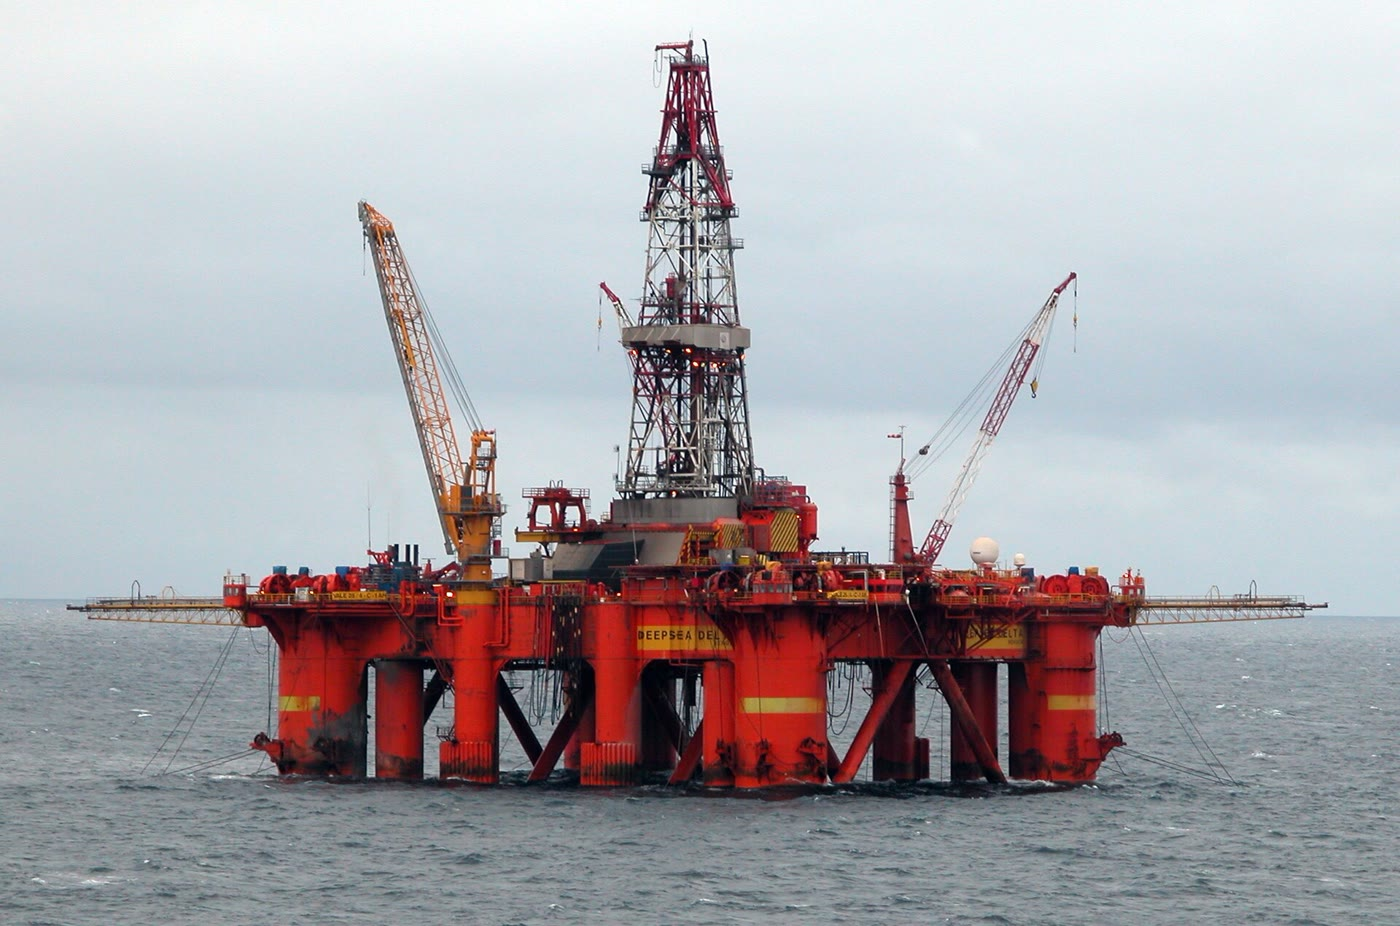
\includegraphics[width=0.66\linewidth]{images/book4/b2-16-drilling-rig.jpg}
\par\smallskip{\small 北海中的半潜式钻井平台。从此类平台钻出的钻孔
可提供厚度、年龄与岩石类型，据此重建盆地的
沉降过程。照片：Erik Christensen, 2005, CC BY-SA 3.0。}
\end{omfigure}

\section{盆地及其沉降的成因}\label{sec:b2:basins-compared:types}

本科一年级分册按盆地所处位置来区分盆地。这里则
按驱动沉降的因素来区分。

\begin{definition}[克拉通内盆地、裂谷盆地与被动大陆边缘盆地]\label{def:b2:basins-compared:types}
称\emph{克拉通内盆地}\index{克拉通内盆地}为宽阔的圆形或椭圆形盆地，位于大
陆内部、远离板块边界，在极长的时间尺度上缓慢沉降，
且无大型断层活动。称\emph{裂谷盆地}\index{裂谷盆地}为由正断层
围限、位于伸展中大陆岩石圈上的盆地；其沉降先随伸展，
后随岩石圈冷却而发生。称\emph{被动大陆边缘盆地}\index{被动大陆边缘盆地}为
沉积楔，向海方向增厚，在裂解之后堆积于大陆边缘，
覆盖在旧裂谷减薄的地壳之上。
\end{definition}

\cref{ch:b2:alpine-orogen}中的\omterm{def:b2:alpine-orogen:foreland}{前陆盆地}补全了这一分类，而沿走滑断层
张开的盆地留给本科三年级分册。盆地底部
下沉的机制有三种：
\begin{itemize}
  \item \emph{机械}减薄：地壳受断层拉伸和减薄时，轻的地壳
        被密度更大的地幔取代，地表下降以恢复均衡；
  \item \emph{热}收缩：岩石圈经伸展或自下方受热后，
        冷却，密度增大并缓慢下沉，历时数千万年；
  \item \emph{加载}：逆冲带或沉积物自身的重量使
        岩石圈向下弯曲；这种挠曲属于本科三年级分册的内容，此处
        只需局地的艾里形式沉积负载即可。
\end{itemize}
\omterm{def:b2:basins-compared:types}{裂谷盆地}兼具前两种机制，被动大陆边缘则从裂谷阶段继承第二种机制，
\omterm{def:b2:alpine-orogen:foreland}{前陆盆地}由第三种机制形成。\omterm{def:b2:basins-compared:types}{克拉通内盆地}的成因认识最少。

\begin{omfigure}
\centering
\begin{tikzpicture}[x=1cm, y=1cm, font=\scriptsize, line join=round,
  sed/.style={fill=yellow!35, draw=black!60, line width=0.3pt},
  crust/.style={fill=orange!25, draw=black!60, line width=0.3pt},
  mlith/.style={fill=green!12, draw=black!60, line width=0.3pt},
  asth/.style={fill=red!12, draw=black!60, line width=0.3pt},
  sea/.style={fill=blue!8, draw=none},
  ttl/.style={anchor=south west, font=\scriptsize\bfseries}]
% (a) intracratonic
\begin{scope}
\fill[asth] (0,-2.4) rectangle (6.6,-1.6);
\fill[mlith] (0,-1.6) rectangle (6.6,-0.7);
\fill[crust] (0,-0.7) -- (6.6,-0.7) -- (6.6,0) -- (4.9,0) .. controls (4.1,-0.45) and (2.5,-0.45) .. (1.7,0) -- (0,0) -- cycle;
\fill[sed] (1.7,0) .. controls (2.5,-0.45) and (4.1,-0.45) .. (4.9,0) -- cycle;
\draw[black!70] (0,0) -- (6.6,0);
\node[ttl] at (0,0.05) {(a) 克拉通内盆地};
\node at (3.3,-1.15) {岩石圈地幔};
\node at (3.3,-2.0) {软流圈};
\end{scope}
% (b) rift
\begin{scope}[xshift=7.2cm]
\fill[asth] (0,-2.4) -- (6.6,-2.4) -- (6.6,-1.6) -- (4.5,-1.6) -- (3.3,-1.0) -- (2.1,-1.6) -- (0,-1.6) -- cycle;
\fill[mlith] (0,-1.6) -- (2.1,-1.6) -- (3.3,-1.0) -- (4.5,-1.6) -- (6.6,-1.6) -- (6.6,-0.7) -- (4.4,-0.7) -- (3.3,-0.45) -- (2.2,-0.7) -- (0,-0.7) -- cycle;
\fill[crust] (0,-0.7) -- (2.2,-0.7) -- (3.3,-0.45) -- (4.4,-0.7) -- (6.6,-0.7) -- (6.6,0) -- (4.6,0) -- (4.25,-0.42) -- (3.75,-0.2) -- (3.35,-0.4) -- (2.95,-0.15) -- (2.45,-0.42) -- (2.0,0) -- (0,0) -- cycle;
\fill[sed] (2.0,0) -- (2.45,-0.42) -- (2.95,-0.15) -- (3.35,-0.4) -- (3.75,-0.2) -- (4.25,-0.42) -- (4.6,0) -- cycle;
\draw[thick] (2.0,0) -- (2.5,-0.5) (4.6,0) -- (4.2,-0.5) (2.95,-0.15) -- (3.4,-0.48);
\draw[black!70] (0,0) -- (6.6,0);
\node[ttl] at (0,0.05) {(b) 裂谷};
\node at (1.45,-1.15) {岩石圈地幔};
\node at (5.4,-2.0) {软流圈};
\end{scope}
% (c) passive margin
\begin{scope}[yshift=-3.3cm]
\fill[asth] (0,-2.4) -- (6.6,-2.4) -- (6.6,-1.2) -- (0,-1.6) -- cycle;
\fill[mlith] (0,-1.6) -- (6.6,-1.2) -- (6.6,-1.0) -- (4.2,-1.05) -- (2.4,-0.75) -- (0,-0.7) -- cycle;
\fill[crust] (0,-0.7) -- (2.4,-0.75) -- (4.2,-1.05) -- (4.2,-0.85) -- (2.6,-0.25) -- (1.6,0) -- (0,0) -- cycle;
\fill[gray!35, draw=black!60, line width=0.3pt] (4.2,-1.05) -- (6.6,-1.0) -- (6.6,-0.85) -- (4.2,-0.85) -- cycle;
\fill[sed] (1.6,0) -- (2.6,-0.25) -- (4.2,-0.85) -- (6.6,-0.85) -- (6.6,-0.55) -- (3.6,-0.45) -- (2.6,-0.05) -- (2.2,0) -- cycle;
\fill[sea] (2.2,0) -- (6.6,0) -- (6.6,-0.55) -- (3.6,-0.45) -- (2.6,-0.05) -- cycle;
\draw[black!70] (0,0) -- (2.2,0);
\draw[blue!60!black] (2.2,0) -- (6.6,0);
\node[ttl] at (0,0.05) {(c) 被动大陆边缘};
\node at (5.4,-0.95) {\tiny 洋壳};
\node at (1.3,-2.0) {软流圈};
\node at (1.3,-1.05) {岩石圈地幔};
\end{scope}
% (d) foreland
\begin{scope}[xshift=7.2cm, yshift=-3.3cm]
\fill[asth] (0,-2.4) -- (6.6,-2.4) -- (6.6,-2.0) -- (0,-1.5) -- cycle;
\fill[mlith] (0,-1.5) -- (6.6,-2.0) -- (6.6,-1.2) -- (0,-0.7) -- cycle;
\fill[crust] (0,-0.7) -- (6.6,-1.2) -- (6.6,-0.55) -- (3.6,-0.4) .. controls (2.0,-0.15) .. (0,0) -- cycle;
\fill[sed] (0,0) .. controls (2.0,-0.15) .. (3.6,-0.4) -- (6.6,-0.55) -- (5.0,0) -- cycle;
\fill[crust, fill=orange!45] (5.0,0) -- (6.6,-0.55) -- (6.6,0.6) -- (6.1,0.6) -- cycle;
\draw[thrust fault] (6.6,-0.55) -- (5.0,0);
\draw[black!70] (0,0) -- (5.0,0);
\node[ttl] at (0,0.05) {(d) 前陆};
\node[anchor=north east, font=\tiny] at (6.55,0.55) {造山带};
\node at (2.2,-1.25) {岩石圈地幔};
\node at (1.5,-2.05) {软流圈};
\end{scope}
\end{tikzpicture}
\par\smallskip{\small 岩石圈示意剖面中的四类盆地（
非按比例；沉积物为黄色，陆壳为橙色，洋壳为灰色）。垂直
夸大程度很大：真实盆地宽数百千米，深几千米至
15 千米。}
\end{omfigure}

北海的\omterm{def:b2:basins-compared:types}{裂谷盆地}是前两种机制的典型例子。地堑
在那里自三叠纪起形成，最后一次主要的拉伸自中侏罗世
持续至白垩纪中期；此后断层趋于平静，盆地中部仍作为宽缓的浅碟形继续下沉，
由白垩、砂岩充填，并在第三纪的大部分时间里又由页岩和
泥岩充填。若仅受水体荷载，其基底在断层停止活动后还将再下沉 1100 至
\qty{1400}{m}（盆地中部）和 600 至 \qty{700}{m}（两翼）。
% ledger: sc80b4:north-sea

美国东部的被动大陆边缘以更大的尺度显示出同样的下沉。
横跨陆架的地震剖面显示，中生代及更新的岩层在
巴尔的摩峡谷海槽中厚度超过 \qty{14}{km}，在乔治浅滩盆地中为 \qty{8}{km}，这些地层单元均向大洋方向增厚。
其侏罗纪沉积中心沿袭了裂谷的构造，
以及后期热沉降的区带。
% ledger: schlee76:atlantic, lang24:atlantic

密歇根盆地是\omterm{def:b2:basins-compared:types}{克拉通内盆地}的典型。盆地呈卵形，面积达数十万
平方千米，其中充填了超过 \qty{4}{km} 的显生宙沉积物，这些沉积物在
约 5 亿年间分几个不同阶段沉积而成，几乎没有断层活动。其快速沉降期与
北美及其他大陆内部的盆地沉降期相吻合，
这表明其成因超出单个盆地的范围。对超过 57\,000
口井的测井资料做\omterm{def:b2:basins-compared:backstripping}{回剥}分析，显示出一种持续时间长、近似圆形的沉降格局，作者认为
地幔下降流可以解释，该格局在大陆远端
边缘两次造山运动期间中断。\omterm{def:b2:basins-compared:types}{克拉通内盆地}为何下沉，目前仍有争议。
% ledger: sloss82:michigan, crowe09:michigan

\section{沉降曲线}\label{sec:b2:basins-compared:curves}

水井或实测剖面给出各地层单元的现今深度、岩石类型和年龄，
年龄由化石或地层对比读取。若再结合各单元沉积时的水深，
其沉积水深由化石与沉积构造读出，便可得到盆地的历史。

\begin{definition}[沉降曲线]\label{def:b2:basins-compared:curve}
盆地在某一地点的\emph{沉降曲线}\index{沉降曲线}，是某一参考面
（通常取基底或最老地层单元的底面）在海平面以下的深度，
随时间变化的图像。\emph{总}沉降曲线采用各时刻当时的沉积物厚度，
再加上水深；\emph{构造}沉降曲线则以水代替沉积物，
并去除其均衡效应。
\end{definition}

地层单元在过去从未像今天这样厚。埋藏之后，其孔隙度减小；颗粒本身
未变，但孔隙水已被挤出。本科一年级分册以阿西定律描述埋深
$z$ 处的孔隙度 $\phi(z) = \phi_0\,e^{-z/c}$，并求得位于
$z_1$ 与 $z_2$ 之间的地层固体厚度，
\[
  T_s = (z_2 - z_1) - \phi_0 c\left(e^{-z_1/c} - e^{-z_2/c}\right),
\]
该固体厚度在地层移动时保持不变。要将某一单元\emph{去压实}至较浅位置，
使其顶面位于 $z_1'$ 时，需求出保持相同固体厚度的底面 $z_2'$。
该方程没有闭式解，但可用不动点迭代
\[
  z_2' \leftarrow z_1' + T_s + \phi_0 c\left(e^{-z_1'/c} - e^{-z_2'/c}\right)
\]
从 $z_2' = z_1' + T_s$ 出发，几步即可收敛。地层单位面积的质量
等于其颗粒的质量加上孔隙水的质量，
\[
  m = \rho_g T_s + \rho_w\,(z_2 - z_1 - T_s),
\]
其中 $\rho_g$ 为颗粒密度；将柱体质量除以其厚度，
即得其平均密度 $\bar\rho_s$。

本章所用岩性为沙、页岩、白垩和泥质砂岩，下表
列出斯克莱特与克里斯蒂（1980）的常数，这些常数已收入一个开源程序。
沙在最大深度处仍保有最多孔隙，白垩失去孔隙最快。
% ledger: pybacktrack:compaction

\begin{center}
\small
\begin{tabular}{lccc}
\hline
岩性 & 颗粒密度（\unit{kg.m^{-3}}） & 表面孔隙度 $\phi_0$ & 衰减长度 $c$（\unit{m}） \\
\hline
沙 & 2650 & 0.49 & 3704 \\
页岩 & 2700 & 0.63 & 1960 \\
白垩 & 2710 & 0.70 & 1408 \\
泥质砂岩 & 2680 & 0.56 & 2564 \\
\hline
\end{tabular}
\end{center}

\section{回剥}\label{sec:b2:basins-compared:backstripping}

总\omterm{def:b2:basins-compared:curve}{沉降曲线}混合了两种成因：造成盆地的作用，以及充填物的重量。
将二者分开，正是下一步骤的目的，它是盆地
分析的核心工具。

\begin{definition}[回剥]\label{def:b2:basins-compared:backstripping}
\emph{回剥}\index{回剥}是对盆地构造沉降历史的重建，
即按由新到老的顺序，逐一移去水井中的各地层单元，
每一步都对剩余地层进行去压实，并去除沉积物与水的荷载的均衡效应，
以求得基底在仅有水覆盖时应处的深度。
\end{definition}

最后一步是均衡计算。本科一年级分册针对充填至海平面的盆地做了这一计算；
一般情形还需计入水深和海平面高度。

\begin{proposition}[艾里回剥]\label{prop:b2:basins-compared:backstrip}
设某一时刻盆地中有厚度为 $S$、平均密度为
$\bar\rho_s$ 的沉积物柱，其上水深为 $W_d$，而海平面高出其现今
水平 $\Delta_{SL}$。在局地均衡条件下，地幔密度为 $\rho_m$，水的密度为 $\rho_w$，则
该时刻的构造沉降（自现今海平面算起）为
\[
  Y = S\,\frac{\rho_m - \bar\rho_s}{\rho_m - \rho_w} + W_d
      - \Delta_{SL}\,\frac{\rho_m}{\rho_m - \rho_w}.
\]
\end{proposition}

\begin{proof}
比较同一岩石圈上的两个柱体，向下取至二者之下的补偿深度。在
第一个柱体中，深为 $W_d$ 的水覆盖在厚为 $S$ 的沉积物之上；第二个柱体中，
水单独充填一深为 $Y'$（自同一海面算起）的盆地。二者质量相等：
\[
  \rho_w W_d + \bar\rho_s S + \rho_m\,(d - W_d - S) = \rho_w Y' + \rho_m\,(d - Y'),
\]
其中 $d$ 为补偿面自海面算起的共同深度。由此
得 $Y'(\rho_m - \rho_w) = S(\rho_m - \bar\rho_s) + W_d(\rho_m - \rho_w)$，即前两项
之和。若海平面比今日高 $\Delta_{SL}$，则多出的水不属于盆地自身的沉降，
去掉这部分水后，受水荷载的基底上升
$\Delta_{SL}\rho_w/(\rho_m - \rho_w)$，其在今海平面以下的深度再减小
$\Delta_{SL}$；二者合计为 $\Delta_{SL}\,\rho_m/(\rho_m - \rho_w)$。
\end{proof}
% ledger: pybacktrack:backstrip

取 $\rho_m = \qty{3330}{kg.m^{-3}}$ 与 $\rho_w = \qty{1030}{kg.m^{-3}}$，一柱
平均密度为 \qty{2300}{kg.m^{-3}} 的沉积物，其厚度中计入构造沉降的比例为 $1030/2300 = 0.45$：
即盆地充填厚度的一半以上，是由其自身重量腾出的空间。
若海平面比今日高 \qty{100}{m}，结果降低 \qty{145}{m}。水深与
古海平面是最弱的数据：化石只给出水深范围，
在斜坡上往往宽达数百米，构造沉降也继承了这一范围。

\begin{method}[水井的回剥法]\label{met:b2:basins-compared:backstrip}
\begin{enumerate}
  \item 自底向上列出各单元，及其顶、底的现今深度、
        岩性常数 $(\rho_g, \phi_0, c)$、顶面年龄，以及
        各年龄时的水深。
  \item 由现今深度计算各单元的固体厚度 $T_s$。
  \item 对于单元 $k$ 顶面的年龄，去掉所有更年轻的单元，
        将单元 $k$ 的顶面置于零深度并去压实；随后将各更老的单元依次
        置于其上方单元之下，并逐一去压实。
  \item 将各厚度相加得 $S$，将各质量相加得平均密度
        $\bar\rho_s = \sum m / S$。
  \item 应用 \cref{prop:b2:basins-compared:backstrip} 求得 $Y$；总沉降为
        $S + W_d$。
  \item 对每个年龄重复上述步骤，由最老至现今；以年龄为横轴，绘制 $Y$ 与 $S + W_d$ 随年龄变化的曲线。
\end{enumerate}
\end{method}

下图给出\omterm{def:b2:basins-compared:types}{裂谷盆地}中一口虚构水井的结果，共取得四个单元的岩心：
即同裂谷砂岩，沉积于断层活动期，年龄介于 165 与 \qty{150}{Ma} 之间；其上为页岩、
白垩与泥质砂岩。今日无需去压实：基底位于 \qty{6030}{m}，
岩柱平均密度为 \qty{2358}{kg.m^{-3}}，故 $Y = \qty{2648}{m}$
在 \qty{100}{m} 水深之下。在 \qty{150}{Ma} 时，仅砂岩去压实至地表，
厚 \qty{2239}{m}，平均密度为 \qty{2055}{kg.m^{-3}}；在 \qty{200}{m} 水深之下，
$Y = \qty{1441}{m}$。总沉降量
为构造沉降的两倍多；构造\omterm{def:b2:basins-compared:curve}{沉降曲线}先是快速下沉，随后下沉趋缓，
这正是裂谷的形态。
% values (script): figdata/bachelor-2/basins.py part numbers (S_150 2239.5, rho_0 2357.9, Y_0 2648.7, Y_150 1442.1); printed from the rounded chain of calc/ch16.py (rho 2358 -> 2648; T 2239, rho 2055 -> 1441), as in the problem

\begin{omfigure}
\centering
% figdata/bachelor-2/basins.py parts stages and fit (invented well)
\begin{tikzpicture}
\begin{axis}[width=0.8\linewidth, height=6.0cm, x dir=reverse, y dir=reverse, xmin=0, xmax=170,
  ymin=0, ymax=6500, xlabel={年龄 (\unit{Ma})}, ylabel={海平面以下深度 (\unit{m})},
  tick label style={font=\scriptsize}, label style={font=\small}, xtick={0,25,...,175},
  xtick pos=bottom, ytick pos=left,
  legend style={at={(0.5,1.04)}, anchor=south, draw=none, font=\scriptsize, legend columns=3,
  /tikz/every even column/.append style={column sep=8pt}}]
\addplot[omThm, line width=1pt, mark=*, mark size=1.6pt] table[x=age_Ma, y=total_m]
  {figdata/out/bachelor-2-basins-stages.dat};
\addlegendentry{总沉降 $S + W_d$}
\addplot[blue!70!black, line width=1pt, mark=square*, mark size=1.6pt] table[x=age_Ma, y=Y_m]
  {figdata/out/bachelor-2-basins-stages.dat};
\addlegendentry{构造沉降 $Y$}
\addplot[black!70, dashed, line width=0.8pt] table[x=age_Ma, y=Y_m]
  {figdata/out/bachelor-2-basins-fit.dat};
\addlegendentry{拉伸模型，$\beta = 1.50$}
\node[font=\scriptsize, anchor=south west] at (axis cs:149,1500) {裂谷作用结束};
\end{axis}
\end{tikzpicture}
\par\smallskip{\small 对一口含四个单元的虚构水井作\omterm{def:b2:basins-compared:backstripping}{回剥}（数据见周末问题）：
各时刻按当时沉积物状况算得的基底深度，以及构造沉降，
并附上拟合于裂谷作用结束时沉降量的\omterm{def:b2:basins-compared:stretching}{拉伸模型}曲线，
（见\cref{sec:b2:basins-compared:stretching}）。}
\end{omfigure}

\begin{omfigure}
\centering
\begin{tikzpicture}[x=1cm, y=0.1cm, font=\scriptsize, line join=round,
  u/.style={draw=black!60, line width=0.3pt}]
% today
\begin{scope}
\fill[blue!8] (0,0) rectangle (1.6,-1.0);
\fill[u, fill=yellow!25] (0,-1.0) rectangle (1.6,-18.0);
\fill[u, fill=green!18] (0,-18.0) rectangle (1.6,-34.1);
\fill[u, fill=gray!25] (0,-34.1) rectangle (1.6,-45.2);
\fill[u, fill=yellow!55] (0,-45.2) rectangle (1.6,-61.3);
\draw[black!70] (0,-61.3) -- (1.6,-61.3);
\node[anchor=south] at (0.8,0.1) {今日};
\node at (0.8,-9.5) {泥质砂岩};
\node at (0.8,-26) {白垩};
\node at (0.8,-39.6) {页岩};
\node at (0.8,-53.2) {砂岩};
\node[anchor=north] at (0.8,-61.5) {\qty{6130}{m}};
\end{scope}
% at 150 Ma
\begin{scope}[xshift=3.0cm]
\fill[blue!8] (0,0) rectangle (1.6,-2.0);
\fill[u, fill=yellow!55] (0,-2.0) rectangle (1.6,-24.39);
\draw[black!70] (0,-24.4) -- (1.6,-24.4);
\node[anchor=south] at (0.8,0.1) {\qty{150}{Ma}};
\node at (0.8,-13.2) {砂岩};
\node[anchor=north] at (0.8,-24.6) {\qty{2439}{m}};
\end{scope}
\draw[-{Latex}, thick] (4.9,-12) -- (6.1,-12) node[midway, above] {卸载};
% water loaded
\begin{scope}[xshift=6.3cm]
\fill[blue!20] (0,0) rectangle (1.6,-14.4);
\draw[black!70] (0,-14.4) -- (1.6,-14.4);
\node[anchor=south] at (0.8,0.1) {仅水体};
\node at (0.8,-7.2) {水};
\node[anchor=north] at (0.8,-14.6) {$Y = \qty{1441}{m}$};
\end{scope}
\draw[black!40, dashed] (-0.3,0) -- (8.2,0);
\node[anchor=west] at (8.2,0) {海平面};
\end{tikzpicture}
\par\smallskip{\small 对虚构水井在 \qty{150}{Ma} 时的\omterm{def:b2:basins-compared:backstripping}{回剥}（深度按比例绘制）：
今日的四个单元；裂谷作用结束时仅余的砂岩，去压实至地表，置于
\qty{200}{m} 水深之下；同一岩石圈仅受水荷载时，其基底位置更高，
因为水比沉积物轻。}
\end{omfigure}

\section{拉伸模型}\label{sec:b2:basins-compared:stretching}

\omterm{def:b2:basins-compared:types}{裂谷盆地}为何先快速下沉、随后缓慢下沉？
1978 年，麦肯齐提出了一个模型，简单到其参数可由一口水井拟合。

\begin{definition}[拉伸模型；拉伸系数；同裂谷沉降与裂后沉降]\label{def:b2:basins-compared:stretching}
盆地的\emph{拉伸模型}\index{拉伸模型}将裂谷作用表示为
一种瞬时、均匀的纯剪切拉伸，作用于整个岩石圈：地壳与地幔
岩石圈以相同系数减薄，热的软流圈被动上涌以填充空间，此后岩石圈冷却。
\emph{拉伸系数}\index{拉伸系数} $\beta$ 为拉伸后区域宽度与拉伸前宽度之比，
等于地壳初始厚度与最终厚度之比。拉伸期间产生的沉降
即\emph{同裂谷沉降}\index{同裂谷沉降}；此后岩石圈冷却
所产生的沉降即
\emph{裂后沉降}\index{裂后沉降}，
亦称热沉降。
\end{definition}

自然界中的拉伸需要有限的时间，通常为数百万年。后来的模型允许拉伸
持续更长时间，但只要拉伸不太缓慢，简单的瞬时版本便能给出沉降，
大体而正确，因为拉伸之后的冷却过程大致相同。
% ledger: sheplev98:model

\begin{omfigure}
\centering
\begin{tikzpicture}[x=0.5cm, y=0.5cm, font=\scriptsize, line join=round]
% before
\begin{scope}
\fill[orange!25, draw=black!60, line width=0.3pt] (0,0) rectangle (4,-2.8);
\fill[green!12, draw=black!60, line width=0.3pt] (0,-2.8) rectangle (4,-10);
\fill[red!12, draw=black!60, line width=0.3pt] (0,-10) rectangle (4,-11.5);
\node at (2,-1.4) {地壳 $t_c$};
\node[align=center] at (2,-6.4) {地幔 \\岩石圈};
\node at (2,-10.75) {软流圈};
\draw[|-|] (-0.4,0) -- (-0.4,-10) node[midway, left] {$a$};
\node[anchor=south] at (2,0.2) {拉伸前：宽度 $\ell$};
\node[anchor=north] at (2,-11.6) {温度自 $0$ 至 $T_1$};
\end{scope}
% after
\begin{scope}[xshift=4.6cm]
\fill[blue!20] (0,0) rectangle (8,-1.0);
\fill[orange!25, draw=black!60, line width=0.3pt] (0,-1.0) rectangle (8,-2.4);
\fill[green!12, draw=black!60, line width=0.3pt] (0,-2.4) rectangle (8,-6.0);
\fill[red!12, draw=black!60, line width=0.3pt] (0,-6.0) rectangle (8,-11.5);
\draw[black!60, dashed] (0,-10) -- (8,-10);
\node at (4,-0.5) {水，深度 $S_i$};
\node at (4,-1.7) {地壳 $t_c/\beta$};
\node at (4,-4.2) {地幔岩石圈 $a/\beta$};
\node[align=center] at (4,-8.0) {软流圈位于 $T_1$，\\被动上涌};
\node[anchor=south west] at (0,-10) {岩石圈旧底界};
\node[anchor=south] at (4,0.2) {拉伸刚结束时：宽度 $\beta\ell$};
\node[anchor=north] at (4,-11.6) {随后冷却、增厚并下沉};
\draw[black!40] (0,0) -- (8,0);
\end{scope}
\end{tikzpicture}
\par\smallskip{\small \omterm{def:b2:basins-compared:stretching}{拉伸模型}（未按比例绘制）：厚度为 $a$ 的岩石圈，
地壳厚 $t_c$ 的岩石圈被拉伸至原宽度的 $\beta$ 倍；地壳与地幔岩石圈各减薄
$\beta$ 倍，软流圈上涌，地表在水下因\omterm{def:b2:basins-compared:stretching}{同裂谷沉降} $S_i$ 而下沉。
此处 $\beta = 2$。}
\end{omfigure}

\begin{proposition}[拉伸模型中的沉降]\label{prop:b2:basins-compared:stretching}
设厚度为 $a$、地壳厚度为 $t_c$ 的岩石圈，其地温线
自地表处 $0$ 至底部软流圈温度 $T_1$ 呈线性；设地壳与地幔
的密度分别为 $\rho_c(1 - \alpha T)$ 与 $\rho_m(1 - \alpha T)$，其中 $\alpha$ 为热
膨胀系数。若其被瞬时拉伸 $\beta$ 倍，且盆地充以
密度为 $\rho_w$ 的水时：
\begin{enumerate}
  \item \omterm{def:b2:basins-compared:stretching}{同裂谷沉降}为
  \[
    S_i = \frac{a\left(1 - \dfrac{1}{\beta}\right)\left[(\rho_m - \rho_c)\dfrac{t_c}{a}
          \left(1 - \dfrac{\alpha T_1 t_c}{2a}\right) - \dfrac{\alpha T_1 \rho_m}{2}\right]}
          {\rho_m(1 - \alpha T_1) - \rho_w};
  \]
  \item 拉伸后经过时间 $t$ 时的\omterm{def:b2:basins-compared:stretching}{裂后沉降}，取级数首项，为
  \[
    S_t = E_0\,\frac{\beta}{\pi}\sin\frac{\pi}{\beta}\left(1 - e^{-t/\tau}\right),\qquad
    E_0 = \frac{4a\rho_m\alpha T_1}{\pi^2(\rho_m - \rho_w)},\qquad
    \tau = \frac{a^2}{\pi^2\kappa},
  \]
  其中 $\kappa$ 为热扩散率，$\tau$ 为岩石圈的\emph{热时间
  常数}\index{热时间常数}。
\end{enumerate}
\end{proposition}
% ledger: pybacktrack:rifting

\begin{proof}
（1）比较拉伸前与拉伸刚结束后的柱体，向下直至旧的
岩石圈底界，即拉伸前地表以下深度 $a$ 处。拉伸前，厚度为
$t_c$ 的地壳与地幔岩石圈的温度为 $T = T_1 z/a$；拉伸后，两者
各减薄 $\beta$ 倍，温度自 $0$ 升至 $T_1$，跨越 $a/\beta$，故水底以下深度 $z'$ 处的点
温度为 $T = T_1\beta z'/a$；其下，位于 $T_1$ 的软流圈
密度为 $\rho_m(1 - \alpha T_1)$；其上，水充满深度 $S_i$。
一层密度为 $\rho(1 - \alpha T)$、$T$ 由 $T_a$ 线性增至 $T_b$ 者，
其质量为 $\rho\,h\,(1 - \alpha(T_a + T_b)/2)$。拉伸前，柱体所含为
\[
  \rho_c t_c\left(1 - \frac{\alpha T_1 t_c}{2a}\right)
  + \rho_m (a - t_c)\left(1 - \frac{\alpha T_1 (a + t_c)}{2a}\right);
\]
拉伸后，柱体所含为水、减薄后的地壳与地幔岩石圈，以及
充满其余深度 $a$ 的软流圈：
\[
  \rho_w S_i + \frac{\rho_c t_c}{\beta}\left(1 - \frac{\alpha T_1 t_c}{2a}\right)
  + \frac{\rho_m (a - t_c)}{\beta}\left(1 - \frac{\alpha T_1 (a + t_c)}{2a}\right)
  + \rho_m(1 - \alpha T_1)\left(a - S_i - \frac{a}{\beta}\right).
\]
由地壳均衡，两者相等。将含 $S_i$ 的项集中于一侧，
另一侧集中因子 $(1 - 1/\beta)$，展开即得公式；其代数推导
见\cref{exo:b2:basins-compared:11}。

（2）拉伸后，板块借热传导冷却，地表保持在 $0$，底部保持在
$T_1$，并趋向其初始的线性剖面。超温满足热
传导方程，顶部与底部取零值，因而是若干项之和，
$b_n\sin(n\pi z/a)\,e^{-n^2\kappa\pi^2 t/a^2}$；各项以各自的时间常数 $\tau/n^2$ 冷却。
散失的热量使柱体收缩 $\alpha\int \Delta T\,\mathrm{d}z$，而额外的水
充填空间，使其按因子 $\rho_m/(\rho_m - \rho_w)$ 进一步下沉。仅奇数项
有贡献；保留第一项（其系数由初始剖面算得），即得
上述表达式。其余各项冷却快九倍或更多，约经过 1000 万年后，
它们使沉降平移一个近乎恒定的量，该量小于 \qty{100}{m}，
对 $\beta$ 由 1.2 至 4，数值见下。
\end{proof}
% values (script): basins.thermal_series vs basins.thermal, tested in tests/bachelor-2/test_basins.py

麦肯齐论文的参数为 $a = \qty{125}{km}$，$T_1 = \qty{1333}{\celsius}$，
$\alpha = \qty{3.28e-5}{K^{-1}}$, $\kappa = \qty{8e-7}{m^2.s^{-1}}$, $\rho_m =
\qty{3330}{kg.m^{-3}}$（\qty{0}{\celsius} 时），$\rho_c = \qty{2800}{kg.m^{-3}}$；
海水密度取 \qty{1030}{kg.m^{-3}}，可得 $\tau = \qty{62.7}{Ma}$，$E_0 = \qty{3207}{m}$。取地壳厚
\qty{35}{km}，\omterm{def:b2:basins-compared:stretching}{同裂谷沉降}为 $S_i = \qty{4334}{m} \times (1 - 1/\beta)$。
% ledger: sheplev98:parameters, pybacktrack:rifting
% values (script): tau_Myr 62.7, E0_m 3206.9, Si_max_m 4333.8

\begin{omfigure}
\centering
% figdata/bachelor-2/basins.py part curves
\begin{tikzpicture}
\begin{axis}[width=0.8\linewidth, height=6.2cm, y dir=reverse, xmin=0, xmax=200, ymin=0,
  ymax=6500, xlabel={拉伸之后的时间 (\unit{Ma})},
  ylabel={构造沉降 (\unit{m})}, tick label style={font=\scriptsize},
  label style={font=\small}, xtick pos=bottom, ytick pos=left]
\addplot[black!45, line width=1pt] table[x=t_Myr, y=b1.2] {figdata/out/bachelor-2-basins-curves.dat};
\addplot[blue!70!black, line width=1pt] table[x=t_Myr, y=b1.5] {figdata/out/bachelor-2-basins-curves.dat};
\addplot[omThm, line width=1pt] table[x=t_Myr, y=b2] {figdata/out/bachelor-2-basins-curves.dat};
\addplot[orange!80!black, line width=1pt] table[x=t_Myr, y=b4] {figdata/out/bachelor-2-basins-curves.dat};
\node[font=\scriptsize, anchor=south west, inner sep=1pt] at (axis cs:150,1225) {$\beta = 1.2$};
\node[font=\scriptsize, anchor=south west, inner sep=1pt] at (axis cs:150,2595) {$\beta = 1.5$};
\node[font=\scriptsize, anchor=south west, inner sep=1pt] at (axis cs:150,3965) {$\beta = 2$};
\node[font=\scriptsize, anchor=south west, inner sep=1pt] at (axis cs:150,5815) {$\beta = 4$};
\draw[black!40, dashed] (axis cs:62.7,0) -- (axis cs:62.7,6500);
\node[font=\scriptsize, anchor=north west] at (axis cs:63,150) {$t = \tau$};
\end{axis}
\end{tikzpicture}
\par\smallskip{\small \omterm{def:b2:basins-compared:stretching}{拉伸模型}的水载沉降，共四个\omterm{def:b2:basins-compared:stretching}{拉伸系数}，
地壳厚 \qty{35}{km}，参数同正文：同裂谷阶跃位于
$t = 0$ 处，随后的裂后曲线
在 $t = \tau$ 时已达到其最终值的 \qty{63}{\percent}。}
\end{omfigure}

该模型的三个特征可用于实际盆地。
\begin{itemize}
  \item 同裂谷阶跃随 $\beta$ 增大，\omterm{def:b2:basins-compared:stretching}{裂后沉降}亦然；但二者
        之比变化很小，因此若模型成立，两部分都指向同一 $\beta$。
  \item \omterm{def:b2:basins-compared:stretching}{裂后沉降}的时间尺度与 $\beta$ 无关：它仅由
        岩石圈厚度决定。经过 $\tau$ 后，热沉降已完成 \qty{63}{\percent}；
        经过 $3\tau$ 后约完成 \qty{95}{\percent}。停止拉张于两
        亿年前的裂谷几乎不再下沉。
  \item 同裂谷项是减薄的轻质地壳与抬升的热软流圈之间的竞争：前者使地表下沉，
        后者则托起地表。地壳较薄时，
        后者占优，拉张使地表抬升（见\cref{exo:b2:basins-compared:10}）。
\end{itemize}

拟合一口井时，裂谷作用结束时的构造沉降给出 $S_i$，因此
$\beta = 1/(1 - S_i/\qty{4334}{m})$（对 \qty{35}{km} 地壳）；随后预测裂后曲线
并与其余\omterm{def:b2:basins-compared:backstripping}{回剥}点比较。在虚构的井中，$S_i = \qty{1441}{m}$
得 $\beta = 1.50$，曲线与较晚各点相差仅数米（图见
\cref{sec:b2:basins-compared:backstripping}）。实际盆地很少如此配合。在
北海中部，拉伸量为 50 至 \qty{100}{\percent}，$\beta$ 由 1.5 至 2，
再现了\omterm{def:b2:basins-compared:stretching}{裂后沉降}的振幅与速率。在美国东部大陆边缘，
仅有一段，即长岛台地，其裂后早期充填层
厚度与均匀拉张预测相符；而在乔治浅滩盆地和巴尔的摩峡谷海槽，
其充填层厚 1.5 至 3 倍，必有其他原因在起作用。
% ledger: sc80b4:north-sea, lang24:atlantic

\section{盆地比较}\label{sec:b2:basins-compared:compared}

下表汇总四类盆地。各曲线在形状与时间尺度上互不相同，而
\omterm{def:b2:basins-compared:curve}{沉降曲线}往往是判断被较年轻岩层掩埋的盆地性质的首要线索。

\begin{center}
\small
\begin{tabular}{>{\raggedright\arraybackslash}p{0.13\linewidth}>{\raggedright\arraybackslash}p{0.19\linewidth}>{\raggedright\arraybackslash}p{0.26\linewidth}>{\raggedright\arraybackslash}p{0.29\linewidth}}
\hline
盆地类型 & 实例 & 厚度与持续时间 & 构造\omterm{def:b2:basins-compared:curve}{沉降曲线}的形状 \\
\hline
裂谷 & 北海中部 & 三叠纪以来的地堑；最后一次拉张为中侏罗世至
白垩纪中期；水载裂后下沉 1.1 至 \qty{1.4}{km} & 快速的同裂谷阶跃，
随后呈指数式减缓，$\tau$ 为数十 Ma \\
被动大陆边缘 & 巴尔的摩峡谷海槽 & 自侏罗纪以来超过 \qty{14}{km} & 与
裂谷相似，裂后部分大；充填层向海增厚 \\
前陆 & 北阿尔卑斯\omterm{def:b2:alpine-orogen:foreland}{磨拉石} & 逆冲前缘处超过 \qty{4}{km}，始新世晚期至
中新世晚期 & 紧靠\omterm{def:b2:alpine-orogen:orogen}{造山带}最深，并随之迁移；其内侧部分最终
被逆冲体掩覆 \\
克拉通内 & 密歇根 & 约 500 Ma 内分期超过 \qty{4}{km} & 缓慢，
伴有分期加快的下沉，远处盆地同步出现 \\
\hline
\end{tabular}
\end{center}
% ledger: sc80b4:north-sea, schlee76:atlantic, poag79:bct, krenmayr99:molasse, schmid04:foreland, sloss82:michigan

\omterm{def:b2:alpine-orogen:foreland}{前陆盆地}在一个向其推进的载荷之下下沉：盆地随\omterm{def:b2:alpine-orogen:orogen}{造山带}一同迁移，
阿尔卑斯段的盆地至少迁移 \qty{210}{km}（越过欧洲克拉通），其内侧部分
最终被逆冲体掩覆并携带，正如亚阿尔卑斯\omterm{def:b2:alpine-orogen:foreland}{磨拉石}
在\cref{ch:b2:alpine-orogen}中所示。裂谷随冷却而减缓，无论其
拉张程度如何。\omterm{def:b2:basins-compared:types}{克拉通内盆地}下沉缓慢而持久，且呈脉动式；拉张
与载荷都不能很好地解释它，这正是其仍为研究问题的原因。
% ledger: schmid04:foreland, sinclair97:trinity, krenmayr99:molasse

\begin{inthelab}[沉降分析]
盆地分析人员用程序完成方法框中的工作。例如，一个开源程序
可把钻井点读作带年龄、深度和岩性的地层单元列表，以及一张
岩性表，表中给出各岩性的颗粒密度、表面孔隙度和衰减长度。其
\omterm{def:b2:basins-compared:backstripping}{回剥}模块对各单元去压实，并返回各年龄处的构造沉降量；
由于古水深只知其范围，用户需给出最小值和最大值，
程序则返回对应的两个沉降量及其平均值。第二个模块作逆向运算：
由构造沉降模型预测过去的水深，并可
与化石加以核对。随后，分析人员拟合\omterm{def:b2:basins-compared:stretching}{拉伸系数}、检验海平面曲线，
并根据数百乃至数千口井绘制整个盆地的沉降图。
\end{inthelab}
% ledger: pybacktrack:modules, crowe09:michigan

\section*{练习}\label{sec:b2:basins-compared:exercises}

除非另有说明，练习数据为：$\rho_m = \qty{3330}{kg.m^{-3}}$，$\rho_c =
\qty{2800}{kg.m^{-3}}$，$\rho_w = \qty{1030}{kg.m^{-3}}$；\omterm{def:b2:basins-compared:stretching}{拉伸模型}取 $a =
\qty{125}{km}$，$T_1 = \qty{1333}{\celsius}$，$\alpha = \qty{3.28e-5}{K^{-1}}$，$\kappa =
\qty{8e-7}{m^2.s^{-1}}$，$\tau = \qty{62.7}{Ma}$，$E_0 = \qty{3207}{m}$；地壳厚 \qty{35}{km}，
则 $S_i = \qty{4334}{m}\times(1 - 1/\beta)$；岩性常数见
\cref{sec:b2:basins-compared:curves}中的表。

\begin{exercise}[$\star$]\label{exo:b2:basins-compared:1}
指出各盆地所属的类型及其沉降的主要成因：(a) 密歇根盆地；
(b) 北海中部；(c) 巴尔的摩峡谷海槽；(d) 北阿尔卑斯\omterm{def:b2:alpine-orogen:foreland}{磨拉石}盆地；
(e) 喜马拉雅山前的印度–恒河平原。
\end{exercise}

\begin{exercise}[$\star$]\label{exo:b2:basins-compared:2}
某盆地充填有平均密度为 \qty{2300}{kg.m^{-3}} 的沉积物，厚 \qty{3.0}{km}。(a) 求其
构造沉降（设沉积物达到海平面）。(b) 若其上覆 \qty{200}{m} 厚的水，
则结果如何？(c) 充填物厚度中，由其自身负荷引起的占比为多少？
\end{exercise}

\begin{exercise}[$\star$]\label{exo:b2:basins-compared:3}
地震折射显示，裂谷中原厚 \qty{35}{km} 的地壳已减薄至 \qty{25}{km}。
(a) 求 $\beta$；(b) 拉伸刚结束时岩石圈厚度为多少？(c) 水下
的\omterm{def:b2:basins-compared:stretching}{同裂谷沉降}为多少？
\end{exercise}

\begin{exercise}[$\star$]\label{exo:b2:basins-compared:4}
(a) 验证 $\tau = \qty{62.7}{Ma}$（$1~\text{Ma} = \qty{3.156e13}{s}$）。(b) 有些程序
取 $\kappa = \qty{1e-6}{m^2.s^{-1}}$，此时 $\tau$ 为多少？(c) 对于
岩石圈厚 \qty{100}{km}、$\kappa = \qty{8e-7}{m^2.s^{-1}}$ 的情形，其值为多少？(d) 求
\omterm{def:b2:basins-compared:stretching}{裂后沉降}在 $\tau$ 之后与 $3\tau$ 之后各已完成的比例。
\end{exercise}

\begin{exercise}[$\star\star$]\label{exo:b2:basins-compared:5}
某页岩层现今位于 \qty{1000}{m} 与 \qty{2000}{m} 之间。(a) 求其
顶部与底部的孔隙度。(b) 求其固体厚度。(c) 求其单位面积质量及
平均密度，孔隙中充满水。
\end{exercise}

\begin{exercise}[$\star\star$]\label{exo:b2:basins-compared:6}
将 \cref{exo:b2:basins-compared:5} 中的页岩带回地表。(a) 对去压实公式
从 $z_2' = T_s$ 出发迭代，直至其变化小于 \qty{1}{m}。(b) 求
其在地表的平均密度。(c) 它原来厚了多少？
\end{exercise}

\begin{exercise}[$\star\star$]\label{exo:b2:basins-compared:7}
北海中部受水负载的基底，在
结束于白垩纪中期、约 \qty{100}{Ma} 前的拉伸之后，下沉了 1100 至 \qty{1400}{m}。(a) 按模型，
经过 \qty{100}{Ma} 后，$\beta = 1.5$ 与 $\beta = 2$ 时的\omterm{def:b2:basins-compared:stretching}{裂后沉降}各为多少？(b) 这些
值是否涵盖观测结果？(c) 模型给出 \qty{1250}{m} 时，$\beta$ 为多少？
取 $\frac{\beta}{\pi}\sin\frac{\pi}{\beta} = 0.4705$（$\beta = 1.6$ 时）及 $0.5204$（$\beta
= 1.7$ 时）的值，并作线性插值。
\end{exercise}

\begin{exercise}[$\star\star$]\label{exo:b2:basins-compared:8}
\omterm{def:b2:basins-compared:stretching}{拉伸模型}中的同\omterm{def:b2:basins-compared:types}{裂谷盆地}不充水，而充填密度为
\qty{2300}{kg.m^{-3}} 的沉积物。(a) 在 $S_i$ 的公式中，何者改变？(b) 计算
沉积物负载的 $S_i$，取 $\beta = 1.5$、地壳厚 \qty{35}{km}，已知公式分子为
$a(1 - 1/\beta)\times\qty{74.69}{kg.m^{-3}}$，且 $\rho_m(1 - \alpha T_1) =
\qty{3184.4}{kg.m^{-3}}$。(c) 与水负载的值相比较。
\end{exercise}

\begin{exercise}[$\star\star$]\label{exo:b2:basins-compared:9}
某经\omterm{def:b2:basins-compared:backstripping}{回剥}分析的井在 \qty{100}{Ma} 时给出 $Y = \qty{2171}{m}$，假定海平面为现今值。(a)
若当时海平面高出 \qty{100}{m}，$Y$ 为多少？(b) 若化石给出的水深
介于 100 与 \qty{500}{m} 之间（而非 \qty{300}{m}），则 $Y$ 的范围为何？(c) 两项
不确定度中何者更大？
\end{exercise}

\begin{exercise}[$\star\star\star$]\label{exo:b2:basins-compared:10}
(a) 由 \cref{prop:b2:basins-compared:stretching} 证明，拉伸使地表上升
而非下沉，其条件为 $(\rho_m - \rho_c)\frac{t_c}{a}\left(1 - \frac{\alpha T_1 t_c}{2a}\right) <
\frac{\alpha T_1\rho_m}{2}$。(b) 略去小项 $\alpha T_1 t_c/(2a)$，求
临界地壳厚度。(c) 用一次迭代加以精化。(d) 在地球上何处
可以找到边张开边隆起的裂谷？
\end{exercise}

\begin{exercise}[$\star\star\star$]\label{exo:b2:basins-compared:11}
(a) 写出 \cref{prop:b2:basins-compared:stretching} 证明中的
第 (1) 部分的均衡关系，并导出 $S_i$ 的公式。(b) 证明：板块回到线性地温线后，
最终精确的\omterm{def:b2:basins-compared:stretching}{裂后沉降}为 $\alpha\rho_m T_1 a(1 - 1/\beta)/(2(\rho_m -
\rho_w))$。(c) 取 $\beta = 2$ 计算该值，并与
第一项公式的最终值相比较。
\end{exercise}

\begin{exercise}[$\star\star\star$]\label{exo:b2:basins-compared:12}
某被动大陆边缘经 $\beta = 2$ 的拉伸后已冷却 \qty{150}{Ma}，其
盆地始终充满平均密度为 \qty{2400}{kg.m^{-3}} 的沉积物，直至海平面。
(a) 求受水负载的\omterm{def:b2:basins-compared:stretching}{裂后沉降}。(b) 裂后沉积物厚度为多少？
(c) 巴尔的摩峡谷海槽早期裂后充填物比均匀拉伸预测的厚 1.5 至 3 倍：
若按此比例，此处的厚度应为多少？(d) 试提出可能的成因。
\end{exercise}

\begin{problem}[{周末问题——井的回剥分析}]\label{pb:b2:basins-compared:1}
在虚构的凯斯特尔盆地中，一口井取得了四个层位的岩心。自下而上：裂谷期沉积的沙层，
年代 165 至 \qty{150}{Ma}，现今位于 \qty{4420}{m} 与 \qty{6030}{m} 之间；页岩层，年代 150
至 \qty{100}{Ma}，现今位于 \qty{3310}{m} 与 \qty{4420}{m} 之间；白垩层，年代 100 至 \qty{60}{Ma}，现今位于
\qty{1700}{m} 与 \qty{3310}{m} 之间；泥质沙层，年代 \qty{60}{Ma} 至今，埋深在海底以下 \qty{0}{m} 与
\qty{1700}{m} 之间。化石给出各层沉积时顶部的水深：
\qty{150}{Ma} 时为 \qty{200}{m}，\qty{100}{Ma} 时为 \qty{300}{m}，\qty{60}{Ma} 时为
\qty{150}{m}；现今为 \qty{100}{m}。取本章岩性表，$\rho_m =
\qty{3330}{kg.m^{-3}}$，$\rho_w = \qty{1030}{kg.m^{-3}}$ 用于海水与孔隙水，海平面
取现今值，并采用本章\omterm{def:b2:basins-compared:stretching}{拉伸模型}，地壳厚 \qty{35}{km}。深度按
四舍五入到米。

\noindent\textbf{第一部分——压实。}
\begin{enumerate}
  \item 求沙层现今顶部与底部的孔隙度。
  \item 求沙层的固体厚度。
  \item 页岩、白垩与泥质沙层的固体厚度分别为 \qty{1011}{m}、
        \qty{1409}{m} 和 \qty{1004}{m}。验算其中一项。
  \item 求各层现今的单位面积质量，然后求整个
        地层柱的平均密度。
  \item 在 \qty{150}{Ma} 时沙层位于海底。对其去压实：从 $z_2' =
        T_s$ 出发迭代，直至变化小于 \qty{1}{m}。
  \item 求去压实后沙层的平均密度。
\end{enumerate}

\noindent\textbf{第二部分——\omterm{def:b2:basins-compared:backstripping}{回剥}。}
\begin{enumerate}[resume]
  \item 求 \qty{150}{Ma} 时的构造沉降 $Y$。
  \item 求今天的构造沉降。为何不需要去压实？
  \item 某程序给出 \qty{100}{Ma} 时 $Y = \qty{2171}{m}$，
        \qty{60}{Ma} 时 $Y = \qty{2453}{m}$。计算自 \qty{150}{Ma} 以来
        三个区间内各自的构造沉降平均速率。
  \item 求今天的总沉降，并将其与构造沉降进行比较。
  \item 今天基底深度中，由沉积物负载引起的比例是多少？
  \item 若 \qty{100}{Ma} 时的海平面比今天高 \qty{100}{m}，则那时的 $Y$
        应为多少？
\end{enumerate}

\noindent\textbf{第三部分——拟合\omterm{def:b2:basins-compared:stretching}{拉伸模型}。}裂谷作用取为瞬时发生，
        并于 \qty{150}{Ma} 结束。
\begin{enumerate}[resume]
  \item 曲线上的哪一点给出\omterm{def:b2:basins-compared:stretching}{同裂谷沉降}？
  \item 求\omterm{def:b2:basins-compared:stretching}{拉伸系数} $\beta$，保留两位小数。
  \item 拉伸刚结束时，地壳与岩石圈的厚度各为多少？
  \item 取 $\beta$ 的近似值，计算 $\frac{\beta}{\pi}\sin\frac{\pi}{\beta}$ 以及最终的
        \omterm{def:b2:basins-compared:stretching}{裂后沉降}。
  \item 预测在 100、60 和 \qty{0}{Ma} 时的 $Y$。
  \item 与\omterm{def:b2:basins-compared:backstripping}{回剥}得到的数值进行比较。
  \item 拟合结果之所以很接近，是因为该井是虚构的。试给出三个理由，说明
        一口真实的井为何不会拟合得这样好。
\end{enumerate}

\noindent\textbf{第四部分——未来 5000 万年。}
\begin{enumerate}[resume]
  \item 在接下来的 \qty{50}{Ma} 内，还将发生多少构造沉降？
  \item 若水深保持为 \qty{100}{m}，
        则在此期间可堆积密度为 \qty{2400}{kg.m^{-3}} 的沉积物多少？
  \item 该盆地已完成其最终\omterm{def:b2:basins-compared:stretching}{裂后沉降}的多大比例？
  \item 其中一半是在何时完成的？
  \item 综上所述，该井记录的\omterm{def:b2:basins-compared:stretching}{拉伸系数}是多少？
\end{enumerate}
\end{problem}
